Các bộ định tuyến Internet duy trì các bảng định tuyến, cho phép chúng quyết định các gói sẽ được gửi đến đích một cách tốt nhất. Các bảng định tuyến được xây dựng từ thông tin được chia sẻ giữa các bộ định tuyến sử dụng Border Gateway Protocol (BGP). Chúng bao gồm danh sách các đường dẫn hoàn chỉnh từ bộ định tuyến được đề cập đến các điểm đến trên Internet. Khi một gói đến bộ định tuyến, bộ định tuyến sẽ kiểm tra để xác định đích đến của gói và tìm kiếm đích trong bảng định tuyến. Bước đầu tiên của đường dẫn trong bảng nhập thích hợp sẽ cho bộ định tuyến biết gói tin sẽ được gửi đi như thế nào. Trong lý thuyết, bộ định tuyến chỉ cần lưu trữ bước đầu tiên trên mỗi đường dẫn để định tuyến các gói chính xác. Tuy nhiên, để tính toán hiệu quả các tuyến đường sử dụng BGP, ta muốn các bộ định tuyến nhận thức được toàn bộ đường dẫn đến từng điểm đến. Từ ngày đầu cảu Internet, tất cả các bộ định tuyến đã hoạt động bằng cách này. Chúng ta có thể sử dụng việc này để đo cấu trúc của Internet.\par
Các bảng định tuyến trong các bộ định tuyến được thể hiện ở cấp độ của các hệ thống tự trị (autonomous systems -ASes). Khi một gói dữ liệu đến một bộ định tuyến trong một hệ thống tự trị, gói dành cho một máy tính cụ thể trong cùng hệ thống tự trị đó, thì hệ thống tự trị có trách nhiệm đưa gói tin đến đích cuối cùng. Tuy nhiên, dữ liệu truyền giữa các hệ thống tự trị được xử lý bởi cơ chế BGP trên Internet. Do đó, cần để BGP biết về việc định tuyến chỉ xuống mức hệ thống tự trị và các bảng BGP được trình bày thuận tiện nhất theo thuật ngữ hệ thống tự trị. Trong thực tế, các hệ thống tự trị thường trùng với các tên miền, hoặc gần như vậy.\par
Hệ thống tự trị được gán số nhận dạng duy nhất. Đường dẫn định tuyến bao gồm một chuỗi các số AS này bao gồm các đường dẫn đến một số lượng lớn đích, chúng ta có thể tạo một hình ảnh của Internet ở cấp hệ thống tự trị bằng cách kiểm tra chúng. Quá trình này rất giống với quy trình được sử dụng cho phương pháp theo dõi được mô tả trong phần trước, được mô tả trong hình \ref{fig:h22}. Đầu tiên chúng ta có được một số bảng định tuyến. Mỗi bảng định tuyến chứa một số lượng lớn các đường dẫn bắt đầu từ một nguồn duy nhất (bộ định tuyến) và sự kết hợp của các đường dẫn này tạo ra một ảnh chụp mạng tốt nhưng không hoàn chỉnh, trong đó các đỉnh là các hệ thống tự trị và các cạnh là các kết nối giữa các hệ thống tự trị. Như với traceroute, điều quan trọng là các bộ định tuyến được sử dụng phải phân tán tốt trên mạng để tránh trùng lặp quá nhiều kết quả, số lượng bộ định tuyến được sử dụng phải càng lớn càng tốt để lấy mẫu các cạnh mạng càng đầy đủ.\par
\begin{figure}[ht]
\centering
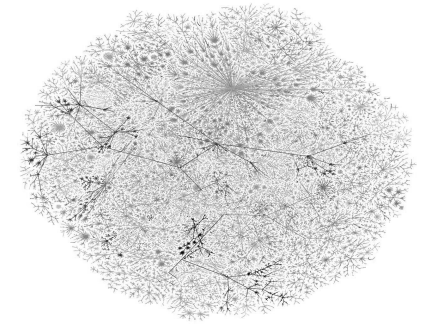
\includegraphics[width=0.5\textwidth]{res/h23.png}
\caption{Cấu trúc của Internet ở cấp độ các hệ thống tự trị. Các đỉnh trong biểu diễn mạng này của Internet là các hệ thống tự trị và các cạnh hiển thị các tuyến đường được lấy bởi dữ liệu truyền đi giữa chúng.}
\label{fig:h23}
\end{figure}
